\begin{figure}[t]
\centering
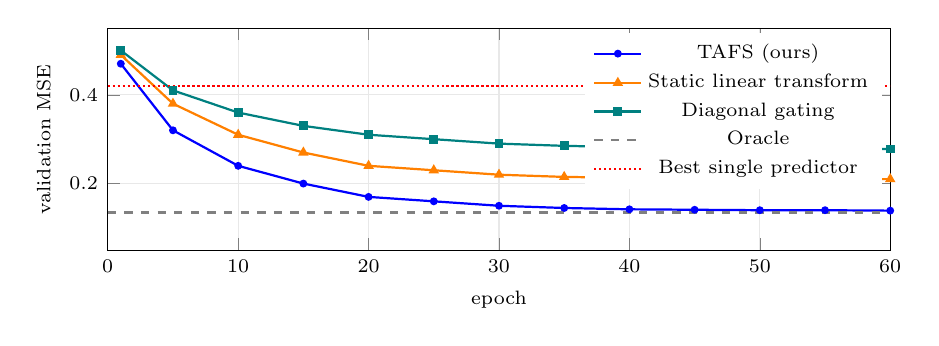
\begin{tikzpicture}
\begin{axis}[
    width=0.95\columnwidth,
    height=4.4cm,
    xlabel={epoch},
    ylabel={validation MSE},
    ymin=0.05, ymax=0.55,
    xmin=0, xmax=60,
    legend style={font=\scriptsize, at={(0.99,0.98)}, anchor=north east, draw=none},
    tick label style={font=\scriptsize},
    label style={font=\scriptsize},
    grid=both,
    grid style={gray!18},
]
\addplot[blue, thick, mark=*, mark size=1pt] coordinates {
(1,0.47)(5,0.32)(10,0.24)(15,0.20)(20,0.17)(25,0.16)(30,0.15)(35,0.145)(40,0.142)(45,0.141)(50,0.140)(55,0.140)(60,0.139)
};
\addlegendentry{TAFS (ours)}
\addplot[orange, thick, mark=triangle*, mark size=1.4pt] coordinates {
(1,0.49)(5,0.38)(10,0.31)(15,0.27)(20,0.24)(25,0.23)(30,0.22)(35,0.215)(40,0.213)(45,0.212)(50,0.211)(55,0.210)(60,0.210)
};
\addlegendentry{Static linear transform}
\addplot[teal, thick, mark=square*, mark size=1.2pt] coordinates {
(1,0.50)(5,0.41)(10,0.36)(15,0.33)(20,0.31)(25,0.30)(30,0.29)(35,0.285)(40,0.282)(45,0.280)(50,0.279)(55,0.278)(60,0.278)
};
\addlegendentry{Diagonal gating}
\addplot[gray, thick, dashed] coordinates {(0,0.135)(60,0.135)};
\addlegendentry{Oracle}
\addplot[red, thick, densely dotted] coordinates {(0,0.42)(60,0.42)};
\addlegendentry{Best single predictor}
\end{axis}
\end{tikzpicture}
\caption{Validation MSE on the synthetic regime-switch task. TAFS approaches the oracle while static-transform baselines plateau well above; the best single base predictor is shown for reference.}
\label{fig:synth_mse}
\end{figure}
